% !TEX encoding = UTF-8 Unicode
\documentclass{proposal}

\title{Proposal: Details}
\author{Steve Clement}
\date{\today}
	
% big font for sections
\usepackage{sectsty}
\sectionfont{\LARGE}

\usepackage{graphicx}
\usepackage{wrapfig}
\usepackage{caption}
\usepackage{subcaption}
\usepackage{pgfgantt}

% \begin{comment} ... \end{comment{}
\usepackage{verbatim}

\setlength{\parskip}{0pt}

\makeatletter
\renewcommand{\paragraph}{
  \@startsection{paragraph}{4}
    {\z@}{1.25ex \@plus 1ex \@minus .2ex}{-1em}
      {\normalfont\normalsize\bfseries}
      }
      \makeatother

\begin{document}

% The following gets pulled from the class file
% Page 1
\newpage

\maketitle

\newpage

% Page 2
\section*{Who are we?}

Coder Dojo is an International movement of technology enthusiasts who believe that there are many ways of engaging youth with Technologies by taking a very practical, hands-on approach.
Specifically in Luxembourg the CoderDojo is powered by CodeClub Luxembourg \footnote{\url{http://www.codeclub.lu}} whose goal is to grow CoderDojo-like efforts all over the Grand-Duchy.

%=================
\section*{Our concept}

\subsection*{Motivation}
For well over 20 years no real progress has been made in educating children in the realm of new technologies.
Whilst these so-called new technologies are not that new anymore, we felt the strong need to provide a regular offer where children can get in touch with technologies in a target appropriate way.
All-tough the Luxembourgish government is also making efforts in approaching children to technologies, our approach is pragmatic, the opposite of a teacher centered course and most of all\ldots FUN

\subsection*{Our idea}
At CoderDojo Luxembourg everything is about real life. The applications, games and other projects we have fun with are all based on real needs. Generally we let the Kids have fun with some very elementary tutorials where they get to know the basics of programming after which we guide them towards their own ideas.

Being based at Level2 has the advantage disposing of an amazing infrastructure where we have not only space to code but also to play around with 3D Printing, soldering of electronics, a vast amount of robotic kits à la (and including) Lego Mindstorms.

The mode of operation is to stimulate the kids creativity in a natural way by letting them fail at first, encourage them to find a solution, talk to the other Dojo members to see if there is a peer who can help and finally mentor them into the right direction once the group (or Google) hasn't found the path.

% Include visual examples of Projects
% Flappy JS, Zombie Conga, Minecraft Py, 
\subsection*{Our current languages taught by mentors}

\begin{figure}[h]
        \centering
                \centering
	  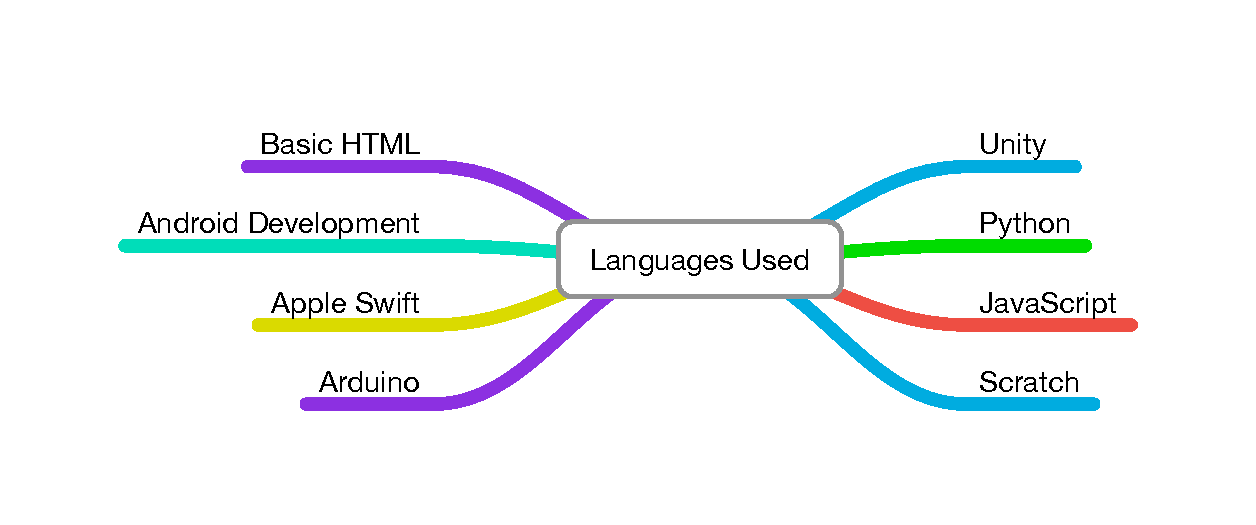
\includegraphics[scale=0.7]{images/LanguagesUsed}
                \caption{Programming Languages Used}
                \label{fig:gull}
\end{figure}

\paragraph{Technologies}
We initiate everyone to the concept of versioning by creating Github \footnote{\url{http://www.github.com}} accounts to keep track of their changes and have a better understanding how their code and the code of their peers has evolved.
% Added Lic. Chooser
\paragraph{License}
Every line of code that is being produced by the Kids will be owned by them, or their legal representative and we encourage them to License their code under any Open Source License \footnote{\url{http://www.licensechooser.lu}} to make the code shareable and re-useable.

\newpage

\paragraph{Roadmap}
In the following months we will use the raised funds to enable an individual to be a part-time employee at the heart of the CoderDojo Luxembourg efforts.
This person will be in charge of creating innovative code content and taking the lead in the weekly CoderDojo's this enabling us to provide a bi-weekly Dojo to accommodate our constantly growing waiting-list.

% Placeholder, replace with GANTT
\begin{center}
\begin{ganttchart}{1}{12}
\gantttitle{2011}{12} \\
\gantttitlelist{1,...,12}{1} \\
\ganttgroup{Group 1}{1}{7} \\
\ganttbar{Task 1}{1}{2} \\
\ganttlinkedbar{Task 2}{3}{7} \ganttnewline
\ganttmilestone{Milestone}{7} \ganttnewline
\ganttbar{Final Task}{8}{12}
\ganttlink{elem2}{elem3}
\ganttlink{elem3}{elem4}
\end{ganttchart}

\end{center}

\paragraph{Focus}
The focus in our exercises will be on first sight very large. The ambition to have very complete sessions is in the nature of technologies as a whole. As they have empowered us to encompass as diverse fields, such as Information security up to Financial technologies, makes us believe that we should integrate as many side-topics as possible.
Needless to say that by stimulating such diverse topics, the reflex to become more independent and eventually delving into the amazing journey of becoming an entrepreneur themselves seems a clear opportunity.
Even-though the Dojo ultimate goal is for the participants to work on their own projects, we will enable the participants to think outside of the box and show them the full range of possibilities.
Numerous were the times in the past where we had discussions about privacy by design, security by design and the responsibilities we have to write better code to solve real-world challenges.


\newpage

% Page 3
\subsection*{Your advantage}
Depending on the chosen sponsorship Level you help us create a viable future for our efforts and whilst everyone agrees it's important to invest into our Future, actually being a real part in this premise.

Further-on this will play an integral part in the economic future of the upcoming work force. Again everyone agrees we need more people going into the technology sector, yet, no real efforts are being made to make this come true.

We will strongly involve you and your company in our efforts giving you ultimate media exposure, including you in our tutorial examples, having your CI in our mobile apps and why not give people at your company the opportunity to volunteer for the Dojo to experience the immense joy of sharing knowledge themselves.

% Show wort example, splash screen for mobile app
\begin{figure}[h]
        \centering
        \begin{subfigure}[b]{0.5\textwidth}
                \centering
	  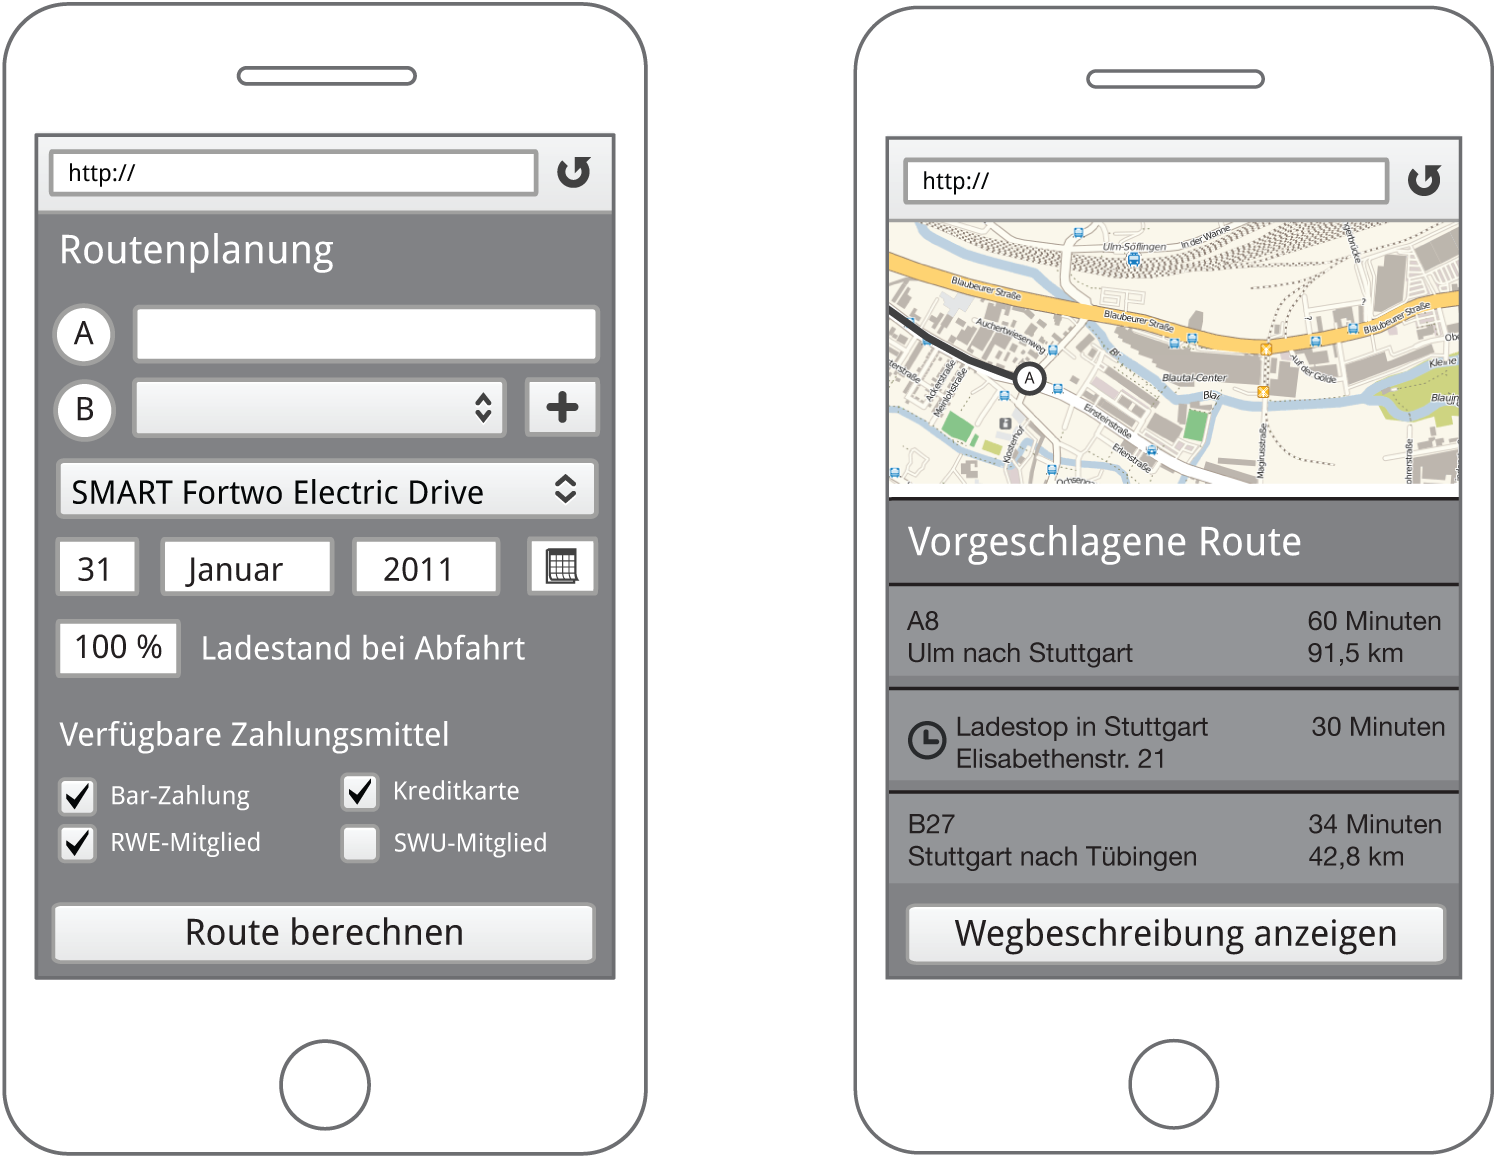
\includegraphics[scale=0.14]{images/phones}
                \caption{Interface Mockup, Smartphone}
                \label{fig:gull}
        \end{subfigure}%
        ~ 
        \begin{subfigure}[b]{0.5\textwidth}
                \centering
                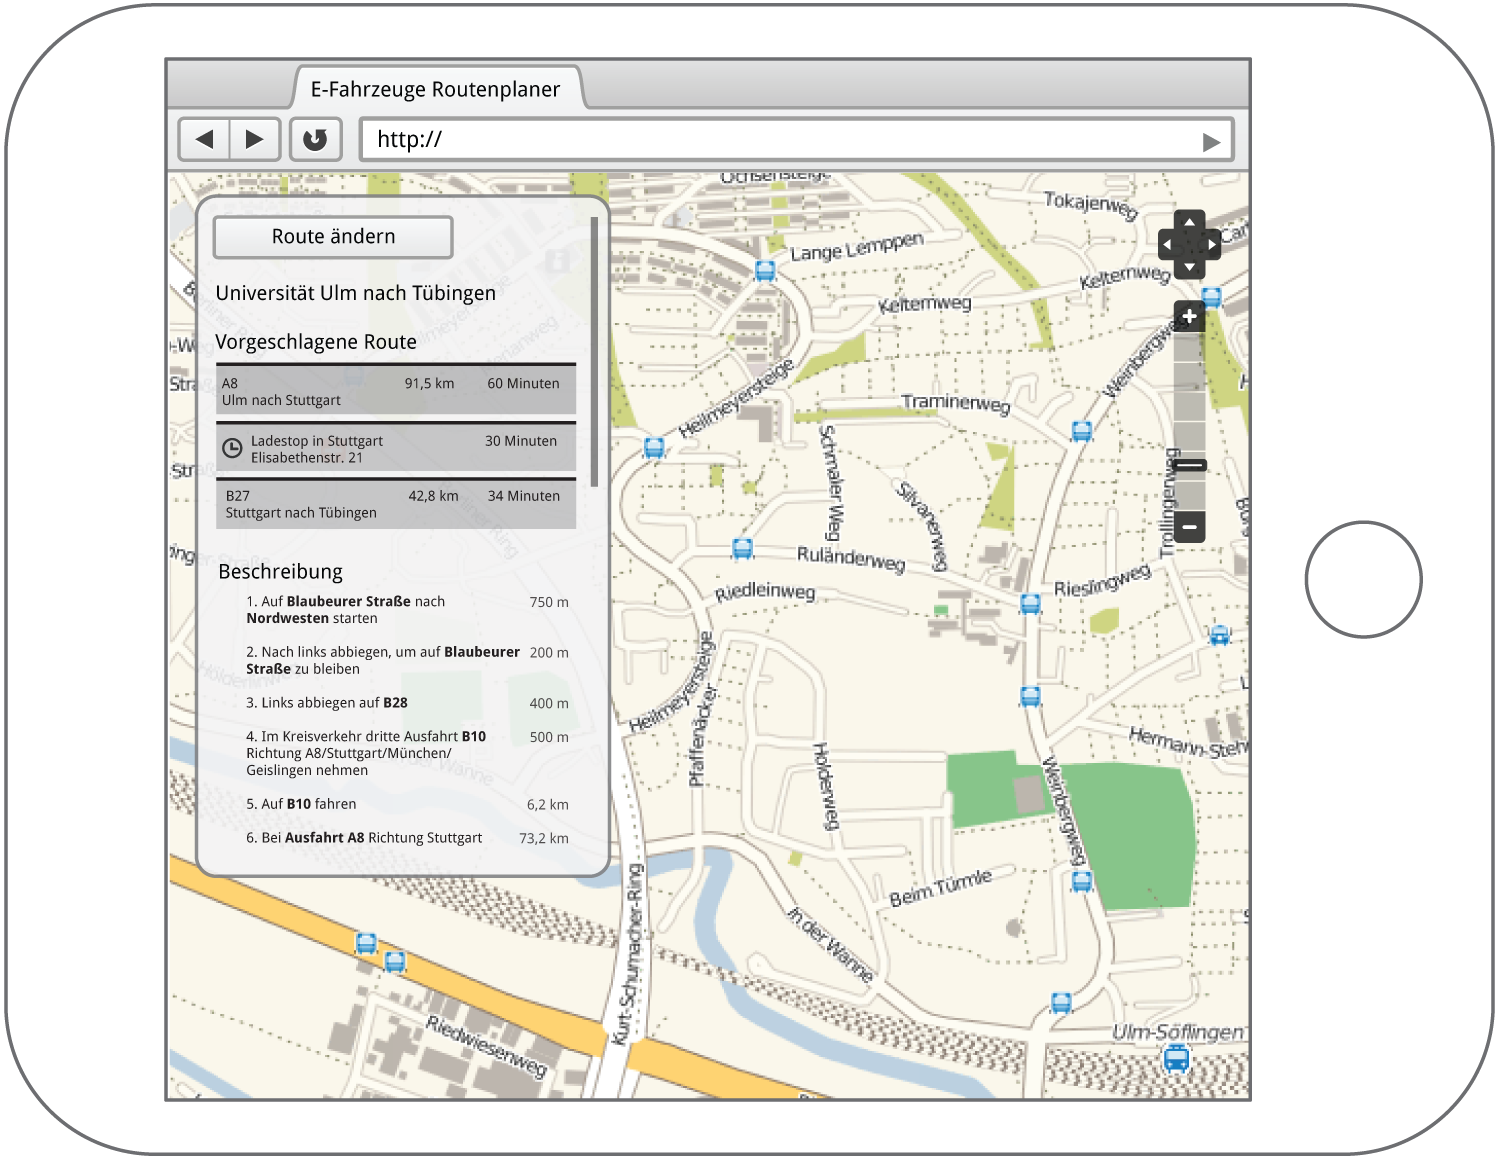
\includegraphics[scale=0.14]{images/tablet}
                \caption{Interface Mockup, Tablet}
                \label{fig:tiger}
        \end{subfigure}
\end{figure}

The above is only one example on how to integrate your CI in our projects. This said bare in mind that this will not be a marketing platform to push particular products but, to a certain extent, push your brand.

\subsection*{Unique advantages}
Being an early adopter in joining our efforts you will be associated in the long term with coding efforts in Luxembourg, thus giving you a first mover advantage.

\section*{CSR}
The more cynical among us might deem CSR as a fancy word for giving back to our society. At CoderDojo we believe that CSR is already an integral part of any successful venture and not only gives to the community being sponsored but also fosters a strong bond within the different teams who are eventually involved in helping the community out.
Further on can CSR help illustrate the real reasons a company adheres to a country and it's current economic model. We would be glad to provide any written statements on the strong partnerships we will forge during our common efforts.

\newpage

% Page 4

%=================
\section*{Packages}

The following sponsorship packages are at your disposal and are not set in stone but can be negotiated on per-need basis and are structured in a crowd-fund matter.

\paragraph{Micro}
The micro package is meant for the individual believers. Not tailored to companies but rather individuals who want to contribute, this will put your name on our website for everyone to see you believe in the project. You will also be invited to any official events and kept up to date what happens at the heart of the Dojo.
42Euro per month

\paragraph{Small}
All of the above plus\ldots
You are a small business with only a minimum of marketing budget. This enables you to get the word out by placing your logo on our website in the sponsorship section.
420Euro per month

\paragraph{Large}
All of the above plus\ldots
Having a solid CSR plan you will be an integral part of the CoderDojo and figure in all our publications, be it press releases, splash screens in our mobile app or communications to the parents.
In addition you will get the opportunity once per year to address the press yourselves with a joint media event where we will review the year in numbers and projects realized.
1000Euro per month

\paragraph{Corporate}
All of the above plus\ldots
You took the big dive into investing into our Kids' future and are the exclusive CoderDojo partner of choice. We will discretely brand the Dojo according to your companies wishes and include your brand in the title of CoderDojo Luxembourg.
We will create a special tutorial only for your company where, again discretely, we will include your CI to enable ultimate exposure and reachability.
A special joint press conference will be held to announce the launch of this new venture and a publication together with the Minister in charge will be held to further reach the press.

2000Euro per month

\ \\

\end{document}
